\documentclass[12pt, twoside]{article}
\usepackage[letterpaper, margin=1in, headsep=0.5in]{geometry}
\usepackage[english]{babel}
\usepackage[utf8]{inputenc}
\usepackage{amsmath}
\usepackage{amsfonts}
\usepackage{amssymb}
\usepackage{tikz}
\usepackage{yhmath}
%\usetikzlibrary{quotes, angles}

\usepackage{graphicx}
\usepackage{enumitem}
\usepackage{multicol}

\usepackage{fancyhdr}
\pagestyle{fancy}
\fancyhf{}
\renewcommand{\headrulewidth}{0pt} % disable the underline of the header

\fancyhead[RE]{\thepage}
\fancyhead[RO]{\thepage \\ Name: \hspace{3cm}}
\fancyhead[L]{BECA / Dr. Huson / 10th Grade Geometry\\* 31 January 2020}

\begin{document}
\subsubsection*{8.4b Exit Note: Area and volume}
 \begin{enumerate}

  \item Use the formulas for the area and circumference of circles:
\[A=\pi r^2\]
\[C=\pi D = 2\pi r\]

  \item Given the circle centered at $O$ with radius $r=3$.
  \begin{multicols}{2}
    \begin{enumerate}
      \item Find the circumference of a circle. %\vspace{1cm}
      \item Find the area of the circle.\vspace{2cm}
    \end{enumerate}
    %\columnbreak
    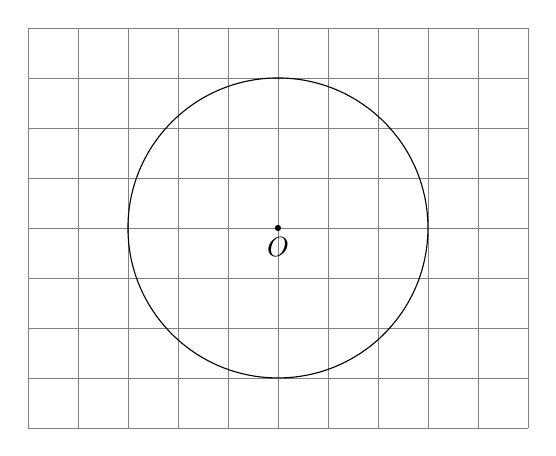
\begin{tikzpicture}[scale=.635]
      \draw [help lines] (-5,-4) grid (5,4);
      %\draw [thick, ->] (-2.2,0) -- (10.4,0) node [below right] {$x$};
      %\draw [thick, ->] (0,-2.2)--(0,10.4) node [left] {$y$};
      \draw (0,0) circle [radius=3] node[below]{$O$};
      \draw [fill] (0,0) circle [radius=0.05];
    \end{tikzpicture}
  \end{multicols}

  \item Find the radius of a circle having an area of $36 \pi$. \vspace{2cm}

\subsubsection*{Model the situation with an equation. Use the formula sheet. You must start with a labeling variable. \hfill Do NOT solve!}

  \item A large concrete post in the shape of a cylinder has a volume of 250 cubic feet. Its height is 12 feet. Find the radius of the base of the post. \vspace{2cm}

  \item A spherical cork fishing net float has a volume of 4000 cubic centimeters. Find its radius. \vspace{2cm}

  \item The volume of a cone having a \textbf{diameter} of 10 inches is 200 cubic inches. Find the cone's height. \vspace{2cm}

\newpage 
\subsubsection*{Vocabulary self-assessment: Circles (fill in the blank with the correct term)}

  \item \textbf{Internal line segments:} Circle with center at point $P$, as shown.
    \begin{multicols}{2}
      \begin{itemize}
        \item  $\overline{AB}$ \quad \rule{3cm}{0.15mm} %Diameter
        \item  $\overline{CP}$ \quad \rule{3cm}{0.15mm} %Radius
        \item  $\overline{DE}$ \quad \rule{3cm}{0.15mm} %Chord
        \item $\angle DPC$ \quad \rule{3cm}{0.15mm} %Central angle 
        \item  $\wideparen{CD}$ \quad \rule{3cm}{0.15mm} %(with measure $m\wideparen{AC} = 72^\circ$)Arc
      \end{itemize}
    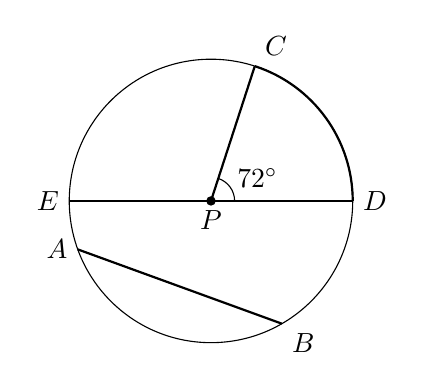
\begin{tikzpicture}[scale=0.6]
      \draw (0,0) circle[radius=3];
      \draw [thick] (3,0) arc (0:72:3);
      \draw [thick] (0:3) node[right] {$D$}--(180:3) node[left] {$E$};
      \draw [thick] (0,0)--(72:3) node[above right] {$C$};
      \draw [thick] (200:3) node[left] {$A$}--(300:3) node[below right] {$B$};
      \fill (0,0) circle[radius=0.1] node[below]{$P$};
      \draw (0.5,0) arc (0:72:0.5) node[right]{$\ 72^\circ$};
      %\draw (35:5) node[right] {$\wideparen{AC}$};
      %\draw (290:5) node[below] {$D$};
    \end{tikzpicture}
  \end{multicols}

  \item \textbf{External lines:} Circle with center at point $O$, at right.
    \begin{multicols}{2}
      \begin{itemize}
        \item  $\overline{FGH}$ \quad \rule{3cm}{0.15mm} %Secant
        \item  $\overline{OG}$ \quad \rule{3cm}{0.15mm} %Radius
        \item  $\overline{FJK}$ \quad \rule{3cm}{0.15mm} %Tangent
        \item $G$ \quad \rule{3cm}{0.15mm} %Point of tangency 
        %\item Note: $\overline{OJ} \perp \overline{FJK}$
      \end{itemize}
    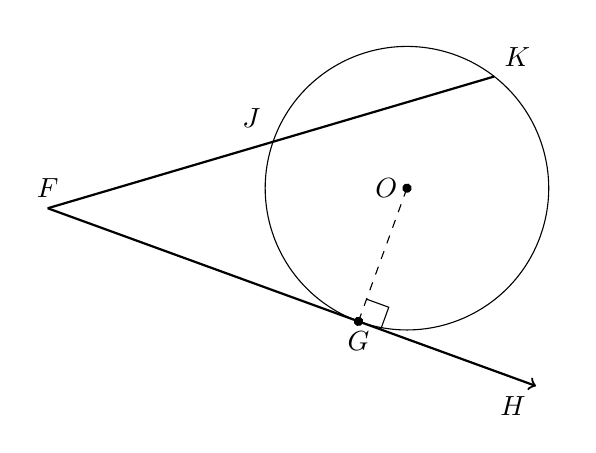
\begin{tikzpicture}[scale=0.6, rotate=-20]
      \draw (0,0) circle[radius=3];
      \draw [thick, ->] (-7,-3) node[above] {$F$}--(4,-3) node[below left] {$H$};
      \draw [thick] (-7,-3)--(72:3) node[above right] {$K$};
      \draw [dashed] (0,-3) node[below] {$G$}--(0,0);
      \fill (0,0) circle[radius=0.1] node[left]{$O$};
      \fill (0,-3) circle[radius=0.1];
      \draw (0,-3) ++(0.5,0)-- ++(0,0.5)--++(-0.5,0);
      \draw (170:3.8) node[below] {$J$};
    \end{tikzpicture}
  \end{multicols}
    
  \item \textbf{Areas:} Circle with center at point $Q$.
    \begin{multicols}{2}
      \begin{itemize}
        \item  $QUV$ \quad \rule{3cm}{0.15mm} %Sector
        \item  $\overline{RS}$ \quad \rule{3cm}{0.15mm} %Diameter
        \item  $RST$ \quad \rule{3cm}{0.15mm} %Semi-circle
      \end{itemize}
    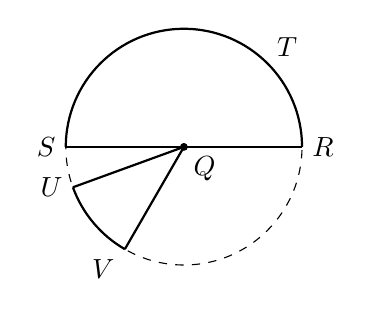
\begin{tikzpicture}[scale=0.5]
      \draw [dashed](0,0) circle[radius=3];
      \draw [thick] (0,0) ++(3,0) arc (0:180:3);
      \draw [thick] (200:3) arc (200:240:3);
      \draw [thick] (0:3) node[right] {$R$}--(180:3) node[left] {$S$};
      \draw [thick] (0,0)--(200:3) node[left] {$U$};
      \draw [thick] (0,0)--(240:3) node[below left] {$V$};
      \fill (0,0) circle[radius=0.1] node[below right]{$Q$};
      \draw (50:3.3) node[right] {$T$};
    \end{tikzpicture}
  \end{multicols}

  \begin{multicols}{2}
  \item \textbf{Polygons and angles in circles:} %Circle with triangle inscribed.
      \begin{itemize}
        \item  $\triangle XYZ$ \vspace{0.5cm} \quad \rule{3cm}{0.15mm} %Inscribed
        \item  $\angle XYZ$ \quad \rule{3cm}{0.15mm} %Inscribed
      \end{itemize} \hspace{1cm}
    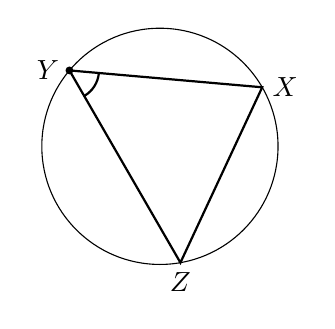
\begin{tikzpicture}[scale=0.5]
      \draw (0,0) circle[radius=3];
      \draw [thick] (140:3) ++(-60:0.75) arc (-60:-5:0.75);
      \draw [thick] (30:3) node[right] {$X$}--(140:3) node[left] {$Y$}
      --(280:3)node[below] {$Z$}--cycle;
      %\draw [thick] (0,0)--(200:3) node[left] {$U$};
      %\draw [thick] (0,0)--(240:3) node[below left] {$V$};
      \fill (140:3) circle[radius=0.1];
      %\draw (50:3.3) node[right] {$T$};
    \end{tikzpicture}
  \end{multicols}


\end{enumerate}
\end{document}
